% -----------------------------------------------------------
%
%  CHAPTER 5  of Quantum information with atoms and photons
%
%  written by many people, Jan 2023
% -----------------------------------------------------------


\section{Two-level atoms and coherent light}
\label{sec:atom_coherent_light}

Consider an system with an atom with only two energy levels, $\ket{g}$ and $\ket{e}$, separated by the quantity $\hbar\omega_{eg}$. A generic state of the system is given by the tensor product of the states in the two subspaces; in particular: 
\begin{align*}
    \ket{\psi_\text{atom}} &\equiv \ket{\psi_A} \in \{\ket{g}, \ket{e}\}  \\
    \ket{\psi_\text{light}} &\equiv \ket{\psi_L}  = \ket{\psi_{k_1}} \otimes \ket{\psi_{k_2}} \otimes  ... \otimes \ket{\psi_{k_L}} \otimes ...  \\
    \ket{\psi} &= \ket{\psi_A} \otimes  \ket{\psi_L}
\end{align*}
For the light state, one can then assume to have all the modes in the vacuum state except for one, leading to the state $\ket{\psi_L} = \ket{0_{k_1}} \otimes \ket{0_{k_2}} \otimes ... \otimes \ket{\psi_{k_L}} \otimes ... $
Then it is possible to assume that the state $\ket{\psi_{k_L}}$ is a coherent state $\ket{\alpha_{k_L}}$, with the following properties:
    \begin{itemize}
        \item there are many photons, which means mathematically that $\left<\hat{n}_{k_L}\right> \equiv \Bar{n} \gg 1$;
        \item the electric field is classical, i.e. with negligible fluctuations, which means that its average value is simply an oscillating function $\langle \hat{\Vec{E}}\rangle= \Vec{\mathcal{E}} \text{cos}(\omega_{k_L} t)$, where $\omega_{k_L} \equiv \omega$ is the only frequency of the problem (this can be derived also from the first propriety). 
    \end{itemize}
From these assumptions, the contributions to the Hamiltonian can be rewritten as:
\begin{align}
    H_\text{atom} &= \hbar \omega_{eg} \ket{e}\bra{e} \\
    H_\text{light} &= \hbar \omega_c \hat{a}^\dagger \hat{a} \\
    H_\text{atom-light} &= - \Vec{\mathcal{E}} \text{cos}(\omega t) \cdot \left[ \Vec{d}_{eg} \ket{e}\bra{g} + \Vec{d}^*_{eg} \ket{g}\bra{e} \right]
\end{align}
where $\Vec{d}_{eg} = \bra{e} \Vec{d} \ket{g}$. One can also introduce the quantity
\begin{align}
    \Omega \equiv \frac{1}{\hbar} \, \Vec{d}_{eg} \cdot \Vec{\mathcal{E}},
\end{align}
called \textit{Rabi frequency}. After this considerations, the complete Hamiltonian becomes
\begin{equation}
    H(t) = \hbar \omega_{eg} \ket{e}\bra{e} + \hbar \Omega \cos(\omega t) \left[  \ket{e}\bra{g} + \text{h.c.} \right]
    \label{eq:Hatom_light}
\end{equation}

In section (\ref{subsec:1.5.2}) the problem of a driven qubit with $\omega \gg \omega_{eg}$ (for both the weak drive case $\omega \gg \Omega$ and the strong drive case $\omega \simeq \Omega$) is solved, but a resolution is possible also for the case $\omega \simeq \omega_{eg}$. This regime is generally indicated with \textit{resonant light condition}. \\
To deal with this situation, it is useful to introduce the \textit{detuning}
\begin{align}
    \delta = \omega_{eg} - \omega.
\end{align}
Hence three energy scales are present and they are associated to three frequencies: $\omega$, $\delta$ and $\Omega$. 


%The resonant light condition brings to $\omega \gg \delta$, but we make the further assumption, later justified, that  $\omega \gg \Omega$.

\subsection{Rotating wave approximation in the high-frequency regime}

Consider a system in which $\omega \gg \delta, \Omega$. To solve the dynamics, one has to go into a new convenient frame, in which the separation of energy scales is visible, which means to find mathematically a new Hamiltonian $$H'(t)= H_0 + V(t).$$
This Hamiltonian can be found going into the \textit{rotating frame}, described by the operator $$R = e^{\text{i} \omega t \ket{e} \bra{e}},$$ from which the new Hamiltonian is given by equation (\ref{eq:transfH}). \\
One can expand the $R$ operator from its definition to find a more convenient representation:
\begin{align}
    R &=  {\mathbb{1} + {i} \omega t \ket{e} \bra{e} + \frac{({i} \omega t)^2}{2 !} \underbrace{(\ket{e} \bra{e})^2}_{\ket{e} \bra{e}} + \sum_{n>2} \frac{(\text{i} \omega t)^n}{n !} \underbrace{(\ket{e} \bra{e})^n}_{\ket{e} \bra{e}} } = \\
     &= \mathbb{1} + \left( {i} \omega t + \frac{({i} \omega t)^2}{2 !} + \sum_{n>2} \frac{({i} \omega t)^n}{n !} \right) \ket{e} \bra{e} = \\
    = & \mathbb{1} + \left( - 1 + \underbrace{ 1 + {i} \omega t + \frac{({i} \omega t)^2}{2 !} + \sum_{n>2} \frac{({i} \omega t)^n}{n !} }_{e^{\text{i} \omega t}} \right) \ket{e} \bra{e} = \\
    = & \mathbb{1} + \left( e^{{i} \omega t} -1 \right) \ket{e} \bra{e}.
\end{align}
We write the contributions to $H'(t)$, i.e.
\begin{align*}
    R \ket{e} \bra{g} R^{\dagger} &=  \left( \mathbb{1} + e^{\text{i} \omega t} -1\right) \ket{e} \bra{g} \left[ \mathbb{1} + \left( e^{\text{i} \omega t} -1 \right) \ket{e} \bra{e}\right]^{\dagger} = \\
    &= e^{\text{i} \omega t} \ket{e} \bra{g} \\
    R \ket{g} \bra{e} R^{\dagger} &=  \left[ \mathbb{1} + \left( e^{\text{i} \omega t} -1 \right) \ket{e} \bra{e}\right] \ket{g} \bra{e} \left( \mathbb{1} + e^{- \text{i} \omega t} -1\right) = \\
    &=  e^{- \text{i} \omega t} \ket{g} \bra{e} \\
    R\Dot{R}^{\dagger} = & \left[ \mathbb{1} + \left( e^{{i} \omega t} -1 \right) \ket{e} \bra{e}\right] \left[ {i} \omega e^{{i} \omega t} \ket{e} \bra{e}\right]^{\dagger} = \\
    &= \left[ -{i} \omega e^{ - i \omega t} - \text{i} \omega + {i} \omega e^{ - {i} \omega t} \right] \ket{e} \bra{e} = \\
    &= - {i} \omega \ket{e} \bra{e}
\end{align*}
and eventually
\begin{align*}
    H'(t) &\equalexpl{\ref{eq:transfH}} R(t) H(t) R^\dagger(t) - i \hbar R(t) \frac{dR^\dagger(t)}{dt} =\\
    &= \hbar\omega_{eg} \ket{e}\bra{e} + \hbar\Omega\cos(\omega t)e^{i\omega t} \ket{e}\bra{g} + \text{h.c.} -i\hbar(-i\omega\ket{e}\bra{e})=\\
    &= \hbar  \delta \ket{e}\bra{e} + \left[\hbar \Omega \cos(\omega t) e^{{i} \omega t} \ket{e}\bra{g} + \text{h.c.} \right] = \\
    &= \hbar  \delta \ket{e}\bra{e} + \left[\hbar \Omega  \frac{e^{ {i} \omega t} + e^{ - {i} \omega t}}{2} e^{ \text{i} \omega t} \ket{e}\bra{g} + \text{h.c.} \right] = \\
    &= \hbar  \delta \ket{e}\bra{e} + \left[ \frac{\hbar  \Omega}{2} \left(1 + e^{ 2 {i} \omega t} \right) \ket{e}\bra{g} + \text{h.c.} \right]
\end{align*}
This Hamiltonian can be rewritten in terms of the time-dependent part $V(t)$ and the time-independent one $H_0$, with
\begin{align}
    H_0 &= {\hbar \delta \ket{e}\bra{e} + \frac{\hbar \Omega}{2} \left[\ket{e}\bra{g} + \ket{g}\bra{e} \right]}   \\ 
    V(t) & = {\frac{\hbar \Omega}{2} \left[e^{2 {i} \omega t} \ket{e}\bra{g} + e^{- 2 {i} \omega t} \ket{g}\bra{e} + \text{h.c.} \right]}. 
\end{align}
To solve the problem, one can use the results obtained in section \ref{sec:time_dep_sys} in the case of a system with a weak drive in the high-frequency regime; this corresponds to the initial assumption $\omega \gg \delta, \Omega$. In particular, it is possible to deduce the final Hamiltonian using (\ref{eq:final_ham}):
\begin{equation}
\label{eq:Hreslight}
    H'= H_0 + \frac{1}{\hbar \omega} \left[V, V^{\dagger}\right] = \hbar \delta \ket{e}\bra{e} + \frac{\hbar \Omega}{2} \left[\ket{e}\bra{g} + \ket{g}\bra{e} \right]
\end{equation}
The term $\left[V, V^{\dagger}\right]$ is responsible for the micro-motion of the system, due to the fact that it goes like $\Omega^2/\omega$. Equation (\ref{eq:Hreslight}) is the final Hamiltonian in the new frame for the resonant light regime ($\omega \gg \delta$, or $\omega \simeq \omega_{eg}$) and in the high-frequency regime ($\omega \gg \Omega$). It is important to notice that we have taken into account only two frequencies ($\Omega$ and $\delta$) in order to study the dynamics of the system. This is the so-called \textit{Rotating-wave approximation}. \\


A final comment is about the fact that, in order to have a simpler notation, one can introduce the following \emph{jump operators}, responsible of the jump from a level to another:
\begin{align}
    \sigma_+ \equiv \ket{e} \bra{g} \qquad \text{and} \qquad \sigma_- \equiv \ket{g} \bra{e}. 
\end{align}
Therefore, the Hamiltonian in the rotating frame with $\omega \gg \delta, \Omega$ is 
\begin{align}
\label{eq:Hrw}
    H = \hbar \delta \ket{e}\bra{e} + \frac{\hbar \Omega}{2} \sigma_+ + \frac{\hbar \Omega}{2} \sigma_-. 
\end{align}


\section{Jaynes-Cummings model for a two-level atom in a cavity}

\begin{figure}[h]
\centering
    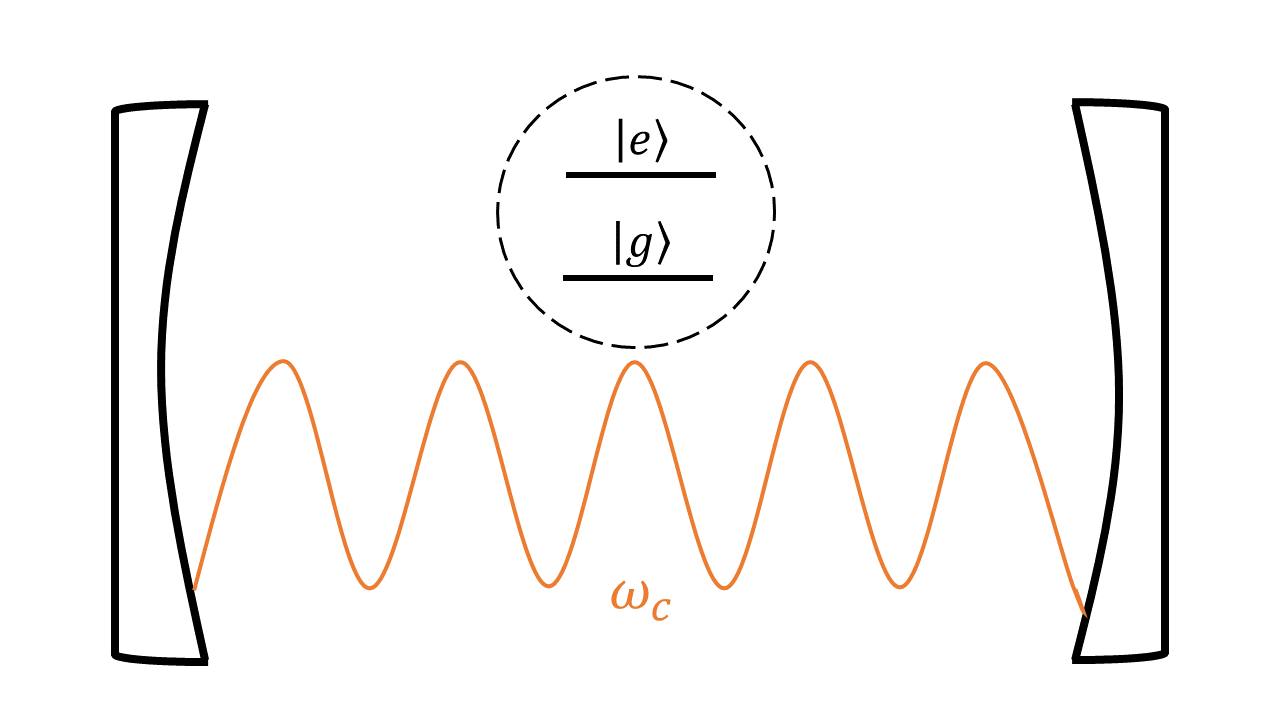
\includegraphics[width=0.65\linewidth]{images/AtomCavity.png}
    \caption{Atom inside the cavity in a quantum regime.}
    \label{fig:atomcavity}
\end{figure}

\subsection{Single-mode cavity}

Consider a cavity with only one mode of the electromagnetic field (\textit{single-mode approximation}) with frequency $\omega_c$ and an atom with only two energy levels; the motion of its center of mass motion can be ignored. The system is presented in figure (\ref{fig:atomcavity}) and the Hamiltonian of this system is made of 
\begin{align*}
    H_\text{light} & = H_{EM} = \hbar \omega_c \crt{} \dsr{} \\
    H_\text{atom} & = H_A = \hbar \omega_{eg} \ket{e}\bra{e} \\
    H_\text{atom-light} & = H_{AL}= -\hat{\Vec{d}} \cdot \hat{\Vec{E}}\\
\end{align*}
Using the expression (\ref{eq:efFP}) for the electric field obtained for a Fabry-Perot cavity for a single mode with frequency $\omega_c = c k_c $ 
\begin{align*}
    \hat{\Vec{E}} = -i \Vec{\epsilon} \sqrt{\frac{\hbar \omega_c}{\varepsilon_0 V}} \sin{(k_c z)} \left( \hat{a}^\dagger - \hat{a} \right), 
\end{align*}
the contribution of the atom-light interaction becomes 
\begin{align*}
    H_{AL} & = - \left( \Vec{d}_{eg} \ket{e}\bra{g} + \Vec{d}^*_{eg} \ket{g}\bra{e} \right) \cdot \left[-i \Vec{\epsilon} \sqrt{\frac{\hbar \omega_c}{\varepsilon_0 V}} \sin(k_c z) \left(\crt{} -  \dsr{}\right)\right] = \\
    &= i \dfrac{\hbar}{2} (\tilde{g} \sigma_{+} + \tilde{g}^{\ast} \sigma_{-}) \left(\crt{} -  \dsr{}\right)
\end{align*}
where the notation previously introduced is used and 
\begin{equation*}
    \tilde{g} = \frac{2\Vec{d}_{eg}^* \cdot \Vec{\epsilon}}{\hbar} \sqrt{\frac{\hbar \omega_c}{\varepsilon_0 V}}  \sin(k_c z)
\end{equation*}
is called \textit{vacuum Rabi frequency}. \\
The total Hamiltonian becomes
\begin{equation}
    H =  \hbar \omega_c \crt{} \dsr{} + \hbar \omega_{eg} \ket{e}\bra{e} + \frac{i \hbar}{2} (\tilde{g} \sigma_{+} +\tilde{g}^{\ast} \sigma_{-}) \left(\crt{} -  \dsr{}\right).
\end{equation}

Consider a situation near resonance regime ($\omega_c \simeq \omega_{eg}$); we know that it is possible to simplify the problem using the rotating-wave approximation, as seen in the previous section. This approximation leads to the elimination of the terms $\sigma_{+} \crt{}$ and $\sigma_{-} \dsr{}$ in $H_{AL}$. More in detail, one can move to a new frame where the energy is conserved through the transformation
\begin{equation}
    R = \underbrace{\exp{{i \omega_{eg} \ket{e}\bra{e} t}}}_{\text{\footnotesize atom}} \, \underbrace{\exp{i \omega_c t \hat{a}^{\dagger} \hat{a}}}_{\text{\footnotesize cavity}} \equiv  R_A \otimes R_{EM}
\end{equation}
Using equation (\ref{eq:transfH}), the new Hamiltonian for the atom-light interaction is 
\begin{align}
    H'_{AL} = \frac{i \hbar}{2} \Tilde{g} \, R \sigma_{+} \hat{a}^{\dagger} R^{\dagger} - \frac{i \hbar}{2} \Tilde{g} \, R \sigma_{+} \hat{a} R^{\dagger} + \text{h.c.}
    \label{eq:atom-light-new}
\end{align}
The first term gives
\begin{align*}
    R \sigma_{+} \hat{a}^{\dagger} R^{\dagger} &= {R_A \sigma_{+} R_A^{\dagger}} \otimes  R_{EM} \hat{a}^{\dagger} R_{EM}^{\dagger} = \\
    &= e^{i \omega_{eg} t } \sigma_{+} \left[  e^{i \omega_c t \hat{a}^{\dagger} \hat{a}} \hat{a}^{\dagger} e^{-i \omega_c t \hat{a}^{\dagger} \hat{a}} \right] 
\end{align*}
and we recognize
\begin{align*}
     e^{i \omega_c t \hat{a}^{\dagger} \hat{a}} \hat{a}^{\dagger} e^{-i \omega_c t \hat{a}^{\dagger} \hat{a}} \equiv  \hat{a}_H^{\dagger}(t)
\end{align*} 
which is the creation operator in the Heisenberg picture for a free harmonic oscillator. Since one can write 
\begin{align*}
    \hat{a}_H^{\dagger}(t) = \hat{a}_H^{\dagger}(0) \, e^{i \omega_c t}, 
\end{align*}
then
\begin{align}
    R \sigma_{+} \hat{a}^{\dagger} R^{\dagger} = e^{i (\omega_{eg} + \omega_c) t} \sigma_{+} \hat{a}_H^{\dagger}(0)
\end{align}
In the same way, one obtains the second term of Eq. \ref{eq:atom-light-new}
\begin{equation}
    R \sigma_{+} \hat{a} R^{\dagger} = e^{i (\omega_{eg} - \omega_c  ) t} \sigma_{+} \hat{a}_H(0)
\end{equation}
Finally, in the in the rotating frame the new Hamiltonian for the atom-light interaction becomes
\begin{equation*}
    H'_{AL}(t) = \underbrace{\frac{i \hbar}{2} \Tilde{g} {e^{i (\omega_{eg} + \omega_c) t}} \sigma_{+} \hat{a}^{\dagger}}_{V^{AL}(t)} + \underbrace{\frac{i \hbar}{2} \Tilde{g} 
    e^{i (\omega_{eg} - \omega_c  )t} \sigma_{+} \hat{a} }_{H^{AL}_0} ~+~ \text{h.c.} 
\end{equation*}
One can notice that the term $H_0$ is independent of time when $\omega_c \simeq \omega_{eg}$, while the term $V(t)$ goes like $e^{2 i \omega_c t}$. Thus, 
\begin{equation*}
    H'_{AL}(t) = \frac{i \hbar}{2} \left[ \tilde{g} e^{2 i \omega_c t} \sigma_+ \hat{a}^\dagger + \tilde{g} \sigma_{+} \hat{a} + \text{h.c.} \right].  
\end{equation*}
The last step consists of going back to the original frame; this leads to 
\begin{align*}
    H_{AL} = -\frac{i \hbar}{2} \tilde{g} \sigma_+ \hat{a} + \frac{i \hbar}{2} \tilde{g}^* \sigma_- \hat{a}^\dagger, 
\end{align*}
from which one can notice that the terms $\sigma_+ \hat{a}^\dagger$ and $\sigma_- \hat{a}$ do not contribute to the dynamics. 
Finally, the rotating-wave approximation is equivalent to the condition
\begin{align*}
    \abs{\omega_{eg} + \omega_c} \gg \abs{\omega_{eg} - \omega_c}, \tilde{g}
\end{align*}
and the total Hamiltonian, which describes the so-called \textbf{Jaynes-Cummings model}, becomes
\begin{align}
    H = \hbar \omega_c \hat{a}^\dagger \hat{a} + \hbar \omega_{eg} \ket{e}\bra{e} -\frac{i \hbar}{2} \tilde{g} \sigma_+ \hat{a} + \frac{i \hbar}{2} \tilde{g}^* \sigma_- \hat{a}^\dagger. 
\end{align}
\\

An alternative form to the model can be obtained by redefining $\Tilde{g} = g e^{i \phi}$, hence
\begin{equation*}
    -i \Tilde{g} \sigma_{+} \hat{a} = g \sigma_{+} \left(-i e^{i\phi} \hat{a} \right) \equiv {g} \sigma_+ \hat{a}',
\end{equation*}
where a unitary transformation allows to introduce $\hat{a}' = -i e^{i\phi} \hat{a}$ and $\hat{a}'^\dagger = i\hat{a}^\dagger e^{-i \phi}$. This implies that $\hat{a}^\dagger \hat{a} = \hat{a}'^\dagger \hat{a}'$ and hence 
\begin{equation} \label{eq:JCModel}
    H = \hbar \omega_c \hat{a}'^\dagger \hat{a}' + \hbar \omega_{eg} \ket{e}\bra{e} + \frac{g \hbar}{2} ( \sigma_+ \hat{a}' + \sigma_- \hat{a}'^\dagger) \qquad \text{with} \qquad g \in \mathbb{R}. 
\end{equation}
This is the model for an atom interacting with a single-mode, nearly resonant ($\omega_{eg} \simeq \omega_{c}$) cavity mode within the rotating-wave approximation, ignoring any dissipation process such as spontaneous emission or any input or output from the cavity.

\subsection{Multi-mode cavity}

To treat a multi-mode, nearly resonant cavity, it is sufficient to consider: 
\begin{align*}
    \sigma_{+} a_n^{\dagger} \quad & \longrightarrow \quad  e^{i(\omega_{eg} + n \omega_c) t} \sigma_{+} a^{\dagger} \\
    \sigma_{+} a_n \quad & \longrightarrow \quad e^{i(\omega_{eg} - n \omega_c) t} \sigma_{+} a
\end{align*}
In this case only $n=1$ would give some relevant terms, the others would be negligible.


\subsection{Dynamics of the Jaynes-Cummings model}

The next step consists of solving the Jaynes-Cummings model; the physics field studying this kind of systems is called \textit{cavity quantum electro-dynamics}.

In order to study the dynamics of the system, one can start from a basis formed with the eigenstates of 
\begin{equation*}
    H_0 = \hbar \omega_c \hat{a}'^\dagger \hat{a}' + \hbar \omega_{eg} \ket{e}\bra{e}. 
\end{equation*}
They are
\begin{align*}
        \ket{g}_A \otimes \ket{n}_{EM} \equiv \ket{g, n} \qquad \text{and} \qquad \ket{e}_A \otimes \ket{n}_{EM} \equiv \ket{e, n}, 
\end{align*}
where $\ket{n}$ is the $n$-photon state in the cavity. 
Taking the atom ground energy as reference value for the zero, the eigenvalues of the eigenstates are given by: 
\begin{align*}
    \ket{g, n} \quad & \longrightarrow \quad E_n^{(g)} = E_A^g + E_{EM}  = 0 + n \hbar \omega_c = \hbar \omega_c n \\
    \ket{e, n} \quad & \longrightarrow \quad E_n^{(e)} = E_A^e + E_{EM}  = \hbar \omega_{eg} + n \hbar \omega_c = \hbar (\omega_{eg}  + \omega_c n )
\end{align*}
These energy levels are reported in figure \ref{fig:JCeigen}, where the decoupling $\delta \equiv \omega_{eg} - \omega_c$ is introduced. 

\begin{figure}[h]
\centering
    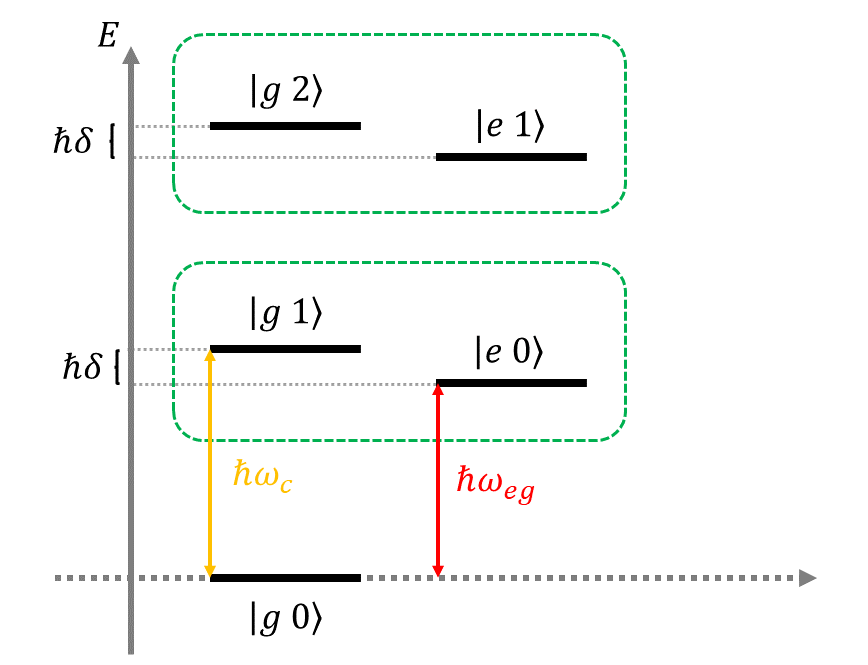
\includegraphics[width=0.57\linewidth]{images/eigenstatesAL.png}
    \caption{Eigenstates of the James-Cummings model (neglecting the atom-light interaction).}
    \label{fig:JCeigen}
\end{figure}

Introducing the interaction between the atom and the cavity, which is described by the last term in Eq. \ref{eq:JCModel}
\begin{equation*}
    H_{AL} = \frac{\hbar g}{2} ({\sigma_{+} \hat{a}} + {\sigma_{-} \hat{a}^{\dagger}}). 
\end{equation*}
the action of this (full) Hamiltonian on the states of the basis is: 
\begin{align*}
    \sigma_+ \hat{a} \ket{g,n} & = \sqrt{n} \ket{e}\bra{g} \ket{g,n-1} = \sqrt{n} \ket{e,n-1}, \\
    \sigma_+ \hat{a} \ket{e,n} & \propto \ket{e}\bra{g} \ket{e,n-1} = 0, \\
    \sigma_- \hat{a}^\dagger \ket{g,n} & \propto \ket{g}\bra{e} \ket{g,n+1} = 0, \\
    \sigma_- \hat{a}^\dagger \ket{e,n} & = \sqrt{n} \ket{g}\bra{e} \ket{e,n+1} = \sqrt{n} \ket{g,n+1}, 
\end{align*}
from which one deduces that $H_{AL}$ only couples 
\begin{align*}
    \ket{g, n} \quad \longleftrightarrow \quad \ket{e,n-1} \qquad \text{and} \qquad 
    \ket{e, n} \quad \longleftrightarrow \quad \ket{g,n+1}. 
\end{align*}
The first relation corresponds to the process of \textit{light absorption}, in which one photon is absorbed by the atom which jumps from the ground state to the excited state, while the second one described the process of \textit{light emission}, in which one photon is emitted from the atom that goes from the excited state to the ground state.

\begin{figure}[t]
\centering
    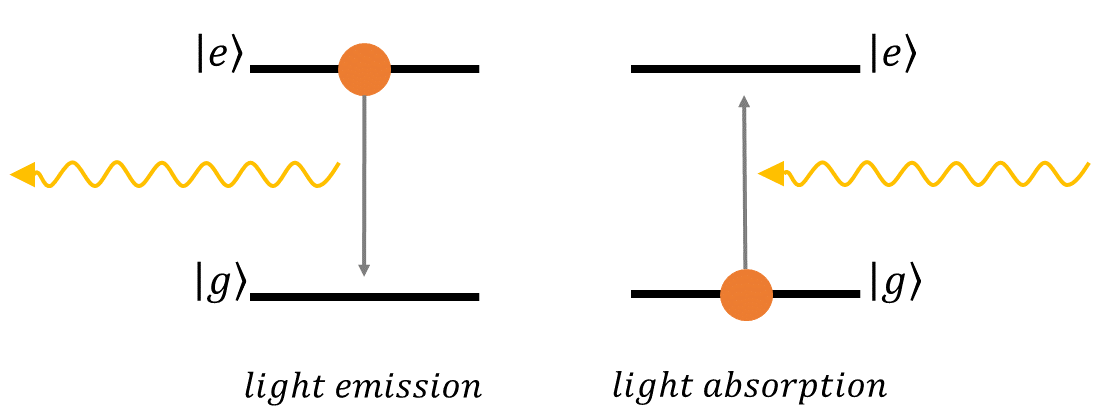
\includegraphics[width=0.67\linewidth]{images/EmsissionAbsorption.png}
    \caption{Processes of light emission and light absorption for an atom with two energy levels: $\ket{g}$ and $\ket{e}$. }
    \label{fig:AbEm}
\end{figure}

The problem ends up being a set of two-levels systems (dotted rectangles in figure \ref{fig:JCeigen}) plus the vacuum state $\ket{g,0}$. Each one of these systems is associated to an Hamiltonian $H_n$ which, in the basis formed by $\ket{g,n}$ and $\ket{e,n-1}$, is given by
\begin{align*}
    H_n & =
    \begin{pmatrix}
    n \hbar \omega_c & \dfrac{g \hbar \sqrt{n}}{2} \\
    \dfrac{\hbar g \sqrt{n}}{2} & \hbar \omega_{eg} +  (n-1) \hbar \omega_c
    \end{pmatrix} = \\ 
        &= n \hbar \omega_c \mathbb{1} + 
        \begin{pmatrix}
            0 & \dfrac{g \hbar \sqrt{n}}{2} \\
            \dfrac{g \hbar \sqrt{n}}{2} & \hbar (\omega_{eg} - \omega_c)
        \end{pmatrix} = \\
        &= n \hbar \omega_c \mathbb{1} +
        \begin{pmatrix} 
            0 & \dfrac{g \hbar \sqrt{n}}{2} \\
            \dfrac{g \hbar \sqrt{n}}{2} & \hbar \delta
        \end{pmatrix}
\end{align*}
Therefore, the total hamiltonian is a $2 \times 2$ block diagonal matrix with the first element of the diagonal being zero (corresponding to $\ket{g, 0}$):
\begin{equation*}
H = \left(
    \begin{array}{ccccc}
     \mathbf{0} &  &  &  \\
     & H_1 &  &  \\
     & & \ddots & \\
     & & & H_n & \\ 
     & & & & \ddots
    \end{array}
\right)
\end{equation*}
As for each $H_n$, one can compute the eigenvalues: 
\begin{equation}
    E_\pm^{(n)} = n \hbar \omega_c + \frac{1}{2} \hbar \delta \pm \frac{\hbar}{2} \sqrt{\delta^2 + g^2 n} \;\;.
    \label{eq:energies}
\end{equation}
This result shows that there is a further separation between $\ket{g, n}$ and $\ket{e, n-1}$, indeed the eigenvectors corresponding to each eigenvalue are 
\begin{align*}
    \ket{+}_n &= \cos \left(\frac{\theta}{2}  \right) \ket{g, n} + \sin\left( \frac{\theta}{2} \right) \ket{e, n-1} \\
    \ket{-}_n &= - \sin\left( \frac{\theta}{2} \right) \ket{g, n} + \cos\left( \frac{\theta}{2} \right) \ket{e, n-1}
\end{align*}
with
\begin{equation*}
    \theta = \arctan \left( \frac{g \sqrt{n}}{\delta}\right).
\end{equation*}
A schematic view of the separation between the eigenstates of the Jaynes-Cumming model is reported in figure \ref{fig:newJCeigen}. 

\begin{figure}[t]
\centering
    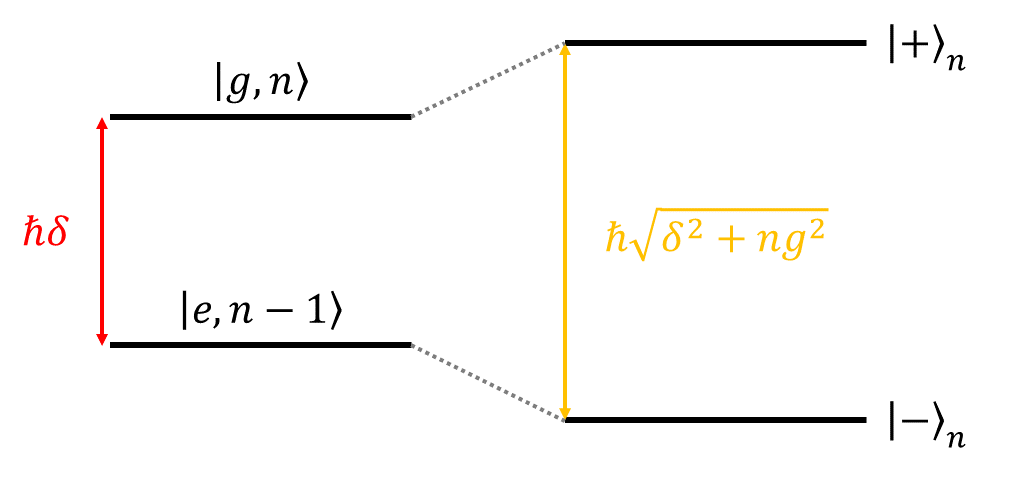
\includegraphics[width=0.6\linewidth]{images/newEigenValue.png}
    \caption{Separation between the eigenstates of the James-Cumming model due to the atom-light interaction.}
    \label{fig:newJCeigen}
\end{figure}

It is important to notice that $\ket{+}_n$ and $\ket{-}_n$ are superpositions of atom and photons modes and they are called \textbf{dressed states}. This superposition is maximum when $\theta = \pi/2$, which is equivalent to the condition $\delta \to 0$ in which $\sin(\theta/2) = \cos{\theta/2}$. When the decoupling is very small, the system is resonant and the separation between eigenvalues, evaluated using (\ref{eq:energies}), becomes $\Delta E_n =  \hbar g \sqrt{n}$. This shows that the Rabi oscillations are now completely quantized since the energy separation between states depends on the number of photons $n$. The separation trend $\omega_n = \Delta E_n$ is reported in figure \ref{fig:omegan}, from which one can notice that the best condition to solve the problem (bigger separation of energies, or lower density) is for low $n$ (far from the classical regime). 

\begin{figure}[h!]
\centering
    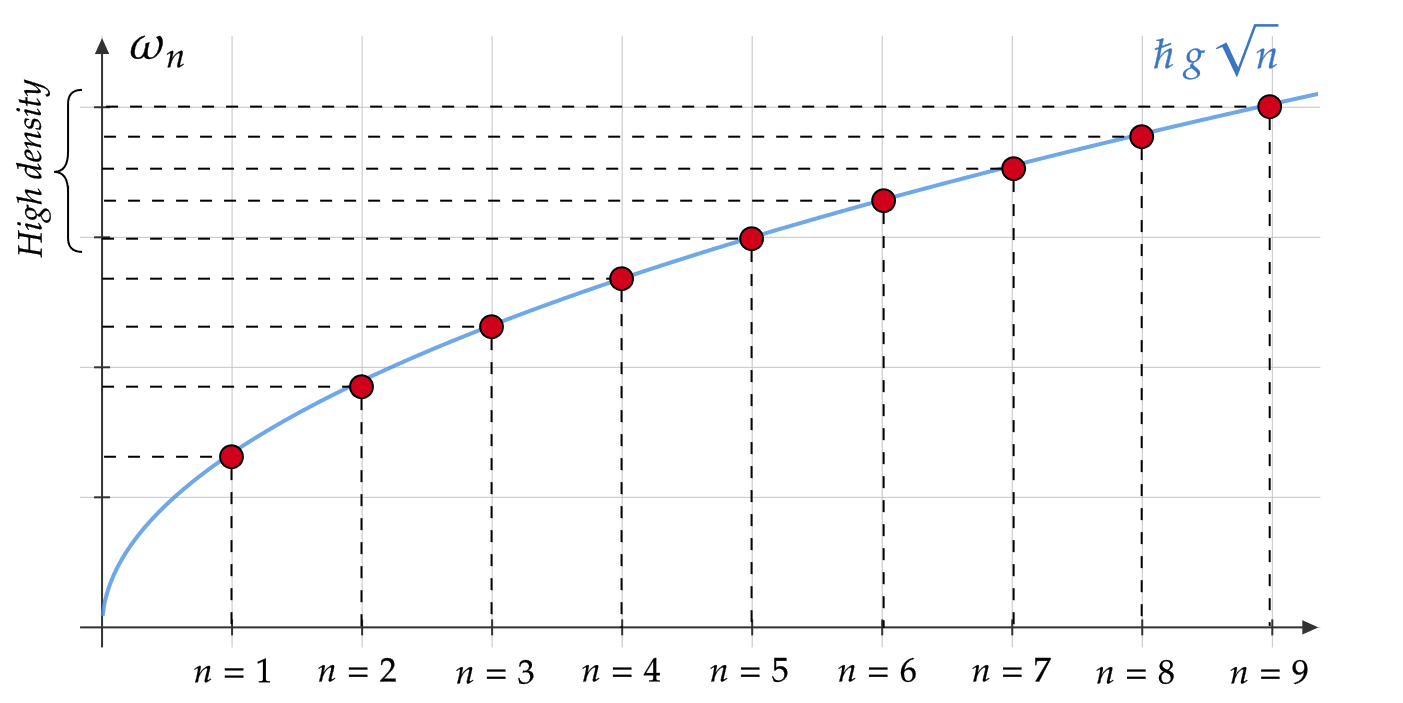
\includegraphics[width=0.8\linewidth]{images/omega_n.png}
    \caption{Frequency associated to the separation of state as a function of the number of photons in the cavity.}
    \label{fig:omegan}
\end{figure}

\subsection{Quantum Rabi oscillations}

Given an initial state $\ket{\psi_0} = \ket{e, n-1} $, it is possible to evaluate the probability that the atom remains in the excited state and the number of photons in conserved (always in the case of a cavity with resonant light, i.e. $\delta \approx 0$): 
\begin{align*}
    P_e^{(n-1)}(t) &\propto \abs{\exp{-iE_+ t/\hbar} + \exp{-iE_- t/\hbar}}^2  \\
    &\propto \abs{\exp{-\frac{i}{2} g \sqrt{n}t } + \exp{\frac{i}{2} g \sqrt{n}t }}^2  \\
    & = \cos^2{\left(\sqrt{n} \, g t\right)}. 
\end{align*}
This trend (shown in Figure \ref{fig:Pe}) represents perfect oscillations, also called \textit{quantum Rabi oscillations}.
% EXPLAIN: only if they are fast compared to the decay time of the system (this happens when the photons exit the cavity). 
\begin{figure}[t]
\centering
    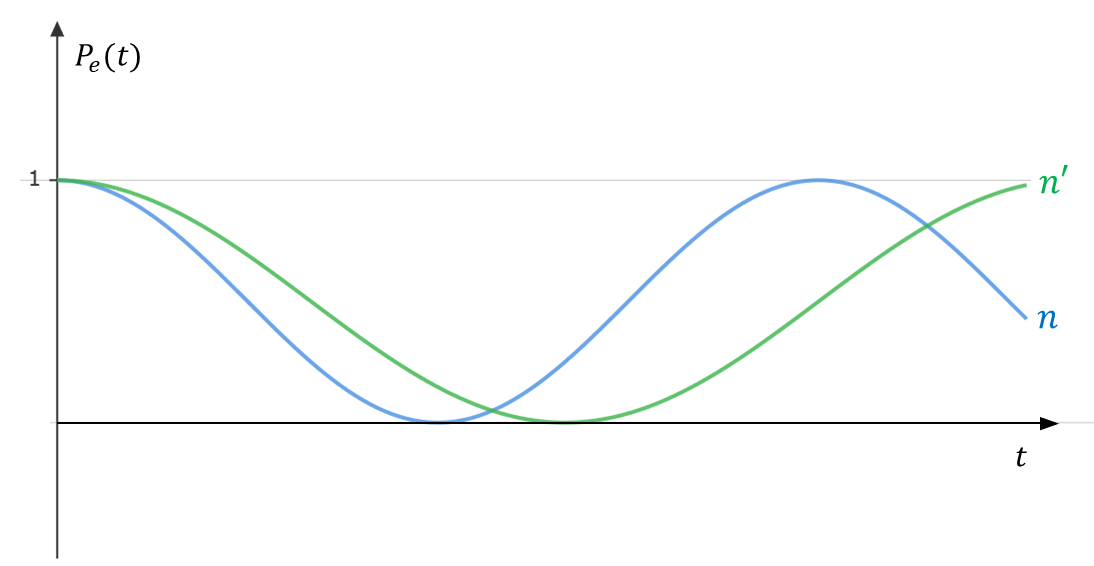
\includegraphics[width=0.7\linewidth]{images/PeJC.png}
    \caption{Probability of finding the atom in the excited state starting from a situation in which the atom is already in the excited state and the number of photons in the cavity are $n$ or $n'$, with $n'<n$. }
    \label{fig:Pe}
\end{figure}

\subsection{Collapses and revivals of the atomic population}

Consider the case in which the initial configuration is $\ket{\psi_0} = \ket{e} \otimes \ket{\alpha}$, with $\ket{\alpha}$ given by equation (\ref{eq:cohstate}), and let $\Bar{n} = \abs{\alpha}^2$. The probability of having an excited state at a time starting from $\psi_0$ is 
\begin{align}
    P_e(t) = |\bra{e}\ket{\psi(t)}|^2 = \sum_{n=1} \abs{c_{n-1}(0)}^2 P_e^{(n-1)}(t), 
    \label{eq:Pe}
\end{align}
where 
\begin{align*}
    \abs{c_{n-1}(0)}^2 = \abs{e^{-\abs{\alpha}^2/2 } \frac{\alpha^{n-1}}{\sqrt{(n-1)!}}}^2 = e^{-\abs{\alpha}^2} \frac{\alpha^{2(n-1)}}{(n-1)!} 
\end{align*} 
indicate the initial occupation probability and $P_e^{(n-1)}$ is similar to the result obtained in the previous section
\begin{align*}
    P_e^{(n-1)} = \cos^2{(\sqrt{\bar{n}+ \delta n} \, gt )}.
\end{align*}
In the last expression, $\delta n$ is introduced to indicate the spread of the distribution which describes the number of photons. Moreover, one can notice that $\delta n/\bar{n} \sim 1/\sqrt{\bar{n}} \to 0$ when $\bar{n} \to \infty$. In this limit, the expression for $P_e^{(n-1)}$ can be rewritten as 
\begin{align*}
    P_e^{(n-1)} & = \cos^2{\left( \sqrt{\bar{n}} gt \sqrt{1 + \frac{\delta n}{\bar{n}}} \right)} \simeq \\
    & \simeq  \cos^2{\left( \sqrt{\bar{n}} gt \left( 1 + \frac{\delta n}{2\bar{n}} \right) \right)} = \\
    & = \cos^2{\left( \sqrt{\bar{n}} gt  + \frac{\delta n}{2\sqrt{\bar{n}}}gt\right)}  = \\
    & = \frac{1}{2} + \frac{1}{2} \cos{\left(2 \sqrt{\bar{n}} g t +  \frac{\delta n}{\sqrt{\bar{n}}}gt \right)} \;\;,
\end{align*}
therefore equation (\ref{eq:Pe}) leads to
\begin{equation*}
    P_e = \frac{1}{2} + \frac{1}{2} \sum_{n=1} \abs{c_{n-1}(0)}^2 \left[ \cos{(2 \sqrt{\bar{n}} gt)} \cos{\left( \frac{\delta n}{\sqrt{\bar{n}}} gt \right)} - \sin{(2 \sqrt{\bar{n}} gt)} \sin{\left( \frac{\delta n}{\sqrt{\bar{n}}} gt \right)}\right]. 
\end{equation*}
Two frequencies are identified from it: 
\begin{align}
    \omega_R \equiv 2 \sqrt{\bar{n}} g \qquad \text{and} \qquad \omega_C \equiv g \frac{\delta n}{\sqrt{\bar{n}}}. 
\end{align}
Having a large average number of photons, one can easily see that $\omega_R \gg \omega_C$ and thus, in the interval $0 < t < (2 \pi)/\omega_C$, only the oscillations with frequency $\omega_R$ are relevant. To better understand what happens, the expression for $P_e(t)$ has to be rewritten in a more convenient form:
\begin{align}
     P_e(t) & = \frac{1}{2} + \frac{1}{2} \sum_{n=0}^\infty e^{-\bar{n}} \frac{\bar{n}^n}{n!} \left[ \cos{\left( 2  \sqrt{\bar{n}} gt + gt \frac{\delta n}{\sqrt{\bar{n}}} \right)}\right] = \label{eq:st1}\\
     &= \frac{1}{2} + \frac{1}{2} \sum_n e^{-\bar{n}} \frac{\bar{n}^n}{n!} \frac{1}{2} \left( \exp{i 2 \sqrt{\bar{n}} gt} \exp{igt\frac{n-\bar{n}}{\sqrt{\bar{n}}}} + \text{c.c.} \right) = \nonumber \\
     & = \frac{1}{2} + \frac{1}{4}\left[ e^{-\bar{n}} \sum_n \left( \frac{\bar{n}^n}{n!} \exp{igt\frac{n}{\sqrt{\bar{n}}}}\right) \exp{i2\sqrt{\bar{n}}gt - igt\frac{\bar{n}}{\sqrt{\bar{n}}}} + \text{c.c.} \right] =  \nonumber\\
     & = \frac{1}{2} + \frac{1}{4} \left[ e^{-\bar{n}} \exp{\bar{n}e^{igt/\sqrt{\bar{n}}}} e^{i \sqrt{\bar{n}}gt} + \text{c.c.} \right] \equalexpl{we develop the exponent of exponent}  \nonumber\\
     & \simeq \frac{1}{2} + \frac{1}{4} \left[ e^{-\bar{n}} \cdot e^{\bar{n}} \, e^{i\sqrt{\bar{n}}gt} \, e^{-g^2 t^2/2} \cdot e^{i\sqrt{\bar{n}}gt} \,  + \text{c.c.} \right] =  \nonumber\\
    &= \frac{1}{2} + \frac{1}{4} \left[ e^{2i\sqrt{\bar{n}}gt} e^{-\frac{1}{2} g^2 t^2} + \text{c.c.} \right] = \nonumber \\
     & = \frac{1}{2} + \frac{1}{2} \cos{\left(2 \sqrt{\bar{n}}gt\right)} e^{-\frac{1}{2}g^2 t^2} \label{eq:stfin}
\end{align}
The cosine term represents the oscillations with frequency $\omega_R$, while the exponential coefficient corresponds to a damping with \textit{collapse time} $\tau_C \sim \sqrt{2}/g$. It is important to underline that the last term does not correspond properly to a damping, but it is better to consider it as a dephasing, since it has been obtained summing over all the possible frequencies. 

\begin{center}
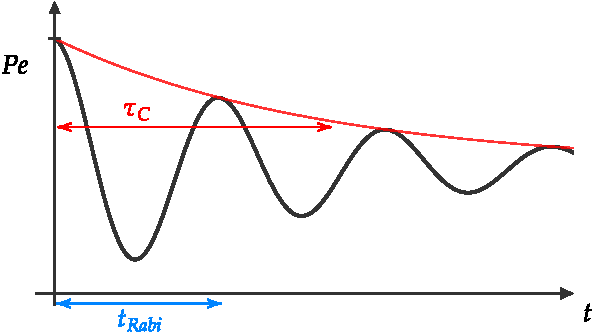
\includegraphics[scale=0.6]{img/Rabi_scales_2.pdf}
\end{center}

From the previous analysis, two time scales have been identified: the one associated to the Rabi frequency ($t_\text{Rabi}$) and the one of the exponential damping ($\tau_C$). In addition to that, there is another time scale that must be considered, which is obtained taking times such that 
\begin{align}
    \frac{gt}{\sqrt{\bar{n}}} = 2 \pi m \qquad \text{with} \qquad m \in \mathbb{N}. 
    \label{eq:revival}
\end{align}
Inserting this value in (\ref{eq:st1}), one obtains $P_e \sim \cos{(4 \pi m\bar{n} + 2 \pi m \delta n)} \sim 1$, and hence the probability reaches again its maximum value every $t$ which satisfies (\ref{eq:revival}), i.e after the so-called \textit{revival time}. An example of the full dynamics is reported in the following figure. 

\begin{center}
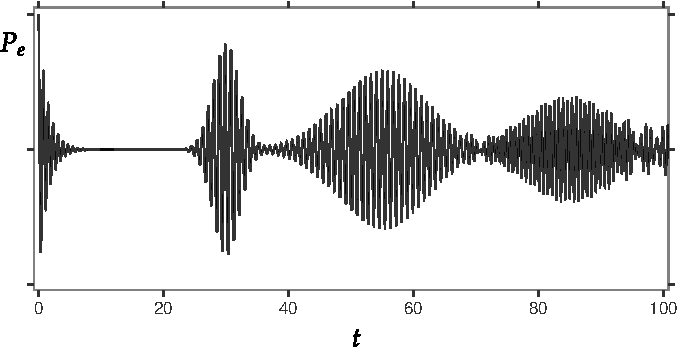
\includegraphics[scale=0.7]{img/Rabi_scales_1.pdf}
\end{center}


\section{Two-level atom coupled with a bath}

Consider a two-level atom coupled with a bath in which many modes are available. This means that, if the atom is in the excited state, there are several decay channels in the bath. The Hamiltonian for this system is made of $H_A$, $H_{EM}$ and $H_{AL}$ which can be written in the rotating-wave approximation
\begin{align}
    H_{AL} = -\vec{d}_{eg} \sigma_+ \hat{\vec{E}}^{(+)} - \vec{d}_{eg}^* \sigma_- \hat{\vec{E}}^{(-)}
\end{align}
with
\begin{align}
    \hat{\vec{E}}^{(+)} &= -i \sum_{\vec{k}, \lambda} \sqrt{\frac{\hbar \omega_k}{2 \varepsilon_0 V}} \vec{\epsilon}_\lambda \,\hat{a}_{\vec{k},\lambda}, \\
    \hat{\vec{E}}^{(-)} &= i \sum_{\vec{k}, \lambda} \sqrt{\frac{\hbar \omega_k}{2 \varepsilon_0 V}} \vec{\epsilon}_\lambda \,  \hat{a}_{\vec{k},\lambda}^\dagger.
\end{align}
These terms correspond to the excitation and de-excitation of the atom after the interaction with light.
This problem can be solved using the Lindblad Master Equation (\ref{eq:cos}) (also called \textit{Nakajima-Zwanzig Equation}) presented in section \ref{sec:ME} and considering
\begin{align*}
    {S'}_\alpha(t') \equiv \sigma_+(t') \qquad  \text{and} \qquad {S'}_\beta^\dagger(t) \equiv \sigma_-(t)
\end{align*}
\begin{align*}
    \hat{B}_\alpha \equiv  i \vec{d}_{eg}^* \cdot \hat{\vec{E}}^{(-)}  \qquad \text{and} \qquad \hat{B}_\beta^\dagger \equiv - i \vec{d}_{eg} \cdot \hat{\vec{E}}^{(+)}. 
\end{align*}
Moreover, 
\begin{align*}
    \sigma_-(t') = \sigma_-(0) \, e^{-i \omega_{eg} t'} \qquad \text{and} \qquad \sigma_+(t) = \sigma_+(0) \, e^{i \omega_{eg} t}. 
\end{align*}
Therefore, the first term of equation (\ref{eq:cos}) becomes
\begin{align*}
    & \int_0^t dt'\, G_{\alpha\beta}(t-t')  \sigma_-(0)  e^{-i \omega_{eg} t'} {\rho'}_S(t') \sigma_+(0)  e^{i \omega_{eg} t} = \\
    & = \int_0^t dt'\,  G_{\alpha\beta}(t-t') e^{i \omega_{eg}(t-t')} \sigma_-(0) \rho'_S(t') \sigma_+(0);
\end{align*}
introducing the variable $\tau \equiv t-t'$ and assuming that $\rho(\tau)$ is smoothly evolving over the time scale at which $G_{\alpha \beta}(\tau)$ decays ($\rho'_S(t-\tau) \simeq \rho'_S(t)$), it can be written as 
\begin{align*}
    - \left[\int_t^0 d\tau \, G_{\alpha \beta}(\tau) e^{i \omega_{eg}\tau} \right]\sigma_- \rho'_S(t) \sigma_+. 
\end{align*}
For the same reason, the lower limit of this integral can be taken $t\to\infty$. Therefore, all the terms in the Master Equation in this assumption has an integral coefficient with the generic form
\begin{align*}
    \mathcal{G}(\omega_{eg}) \equiv \int_0^\infty d \tau \, G_{--}(\tau) e^{i \omega_{eg} \tau} \qquad \text{with} \qquad G_{--}(\tau) = \langle \left( \vec{d}_{eg} \cdot \hat{\vec{E}}^{(+)}(\tau) \right) \left( \vec{d}_{eg}^* \cdot \hat{\vec{E}}^{(-)}(0)\right)  \rangle_B  
\end{align*}
An element of this expectation value can be written as 
\begin{align*}
    \langle \hat{a}_{\vec{k},\lambda}(\tau) \hat{a}^\dagger_{\vec{k}',\lambda'}(0)\rangle_B &= \langle e^{-i \omega_k t} \hat{a}_{\vec{k},\lambda}(0) \hat{a}^\dagger_{\vec{k}',\lambda'}(0)\rangle_B = \\ &= \langle \hat{a}_{\vec{k},\lambda}(0) \hat{a}^\dagger_{\vec{k}',\lambda'}(0)\rangle_B = \\
    & = \delta_{\vec{k},\vec{k}'} \delta_{\lambda,\lambda'} \left(\mathbb{1}-\langle \hat{a}^\dagger_{\vec{k}',\lambda'} \hat{a}_{\vec{k},\lambda}(0)\rangle_B\right). 
\end{align*}
The term $\langle \hat{a}^\dagger_{\vec{k}',\lambda'}\hat{a}_{\vec{k},\lambda}(0)\rangle_B$ can be ignored since it corresponds to the average number of background photons in the bath (like the CMB = cosmic microwave background). Therefore, 
\begin{align}
    \langle \hat{a}_{\vec{k},\lambda}(\tau) \hat{a}^\dagger_{\vec{k}',\lambda'}(0)\rangle_B \simeq \delta_{\vec{k},\vec{k}'} \delta_{\lambda,\lambda'}
\end{align}
and 
\begin{align*}
    \qquad G_{--}(\tau) = \frac{\hbar \omega_k}{2 \varepsilon_0 V} \sum_{\vec{k},\lambda} e^{-i\omega_k t} \left( \vec{d}_{eg} \cdot \vec{\epsilon}_\lambda \right)\left( \vec{d}_{eg}^* \cdot \vec{\epsilon}_\lambda \right). 
\end{align*}
Using the continuum limit to rewrite the summation over $\vec{k}$ and considering the projections of $\vec{d}_{eg}$ and $\vec{d}_{eg}^*$ on $\vec{\epsilon}_1$ and $\vec{\epsilon}_2$, one as 
\begin{align*}
    \qquad G_{--}(\tau) &= \frac{\hbar \omega_k}{2 \varepsilon_0 V} \frac{1}{(2\pi)^2} \int d^3 \vec{k} \, e^{-i\omega_k t} \sum_\lambda \abs{({d}_{eg})_\lambda}^2 = \\
    & = \frac{\hbar \omega_k}{2 \varepsilon_0 V} \frac{1}{(2\pi)^2} \int d^3 \vec{k} \, e^{-i\omega_k t}  \abs{\vec{d}_{eg}}^2 \sin^2{\theta}, 
\end{align*}
where $\theta$ is the angle between $\vec{d}_{eg}$ and the plane of $\vec{\epsilon}_1$ and $\vec{\epsilon}_2$. From this result, the spherical coordinates (with the solid angle $d \Omega$) can be used to rewrite the integral over $d^3 \vec{k}$ and the complete expression is 
\begin{align*}
    \mathcal{G}(\omega_{eg}) 
    &= \int_0^\infty d \tau \, \int \frac{d \Omega}{(2 \pi)^3} \sin^2 \theta \int_0^\infty dk \, k^2 \frac{\hbar \omega}{2 \varepsilon_0} e^{-i(\omega-\omega_{eg})\tau} |{\vec{d}_{eg}}|^2 = \\
    &= \frac{\hbar c |{\vec{d}_{eg}}|^2 }{2 \varepsilon_0 (2\pi)^3} \int d\Omega \, \sin^2 \theta \int_0^\infty dk \, k^3 \int_0^\infty d \tau \, e^{-i(\omega-\omega_{eg})\tau} = \\
    &= \frac{2 \hbar |{\vec{d}_{eg}}|^2  }{3 \varepsilon_0 (2 \pi)^3 c^3} \int_0^\infty d\omega \, \omega^3 \int_0^\infty d\tau \, e^{-i(\omega-\omega_{eg})\tau}, 
\end{align*}
where the relation $\omega_k \equiv \omega = c k$ is used. The last integral is quite tricky. In the following, we will consider its real and imaginary parts.\\
To write the complete Master Equation, the other correlators (similar to $G_{\alpha \beta}$) should be taken into account; it is possible to prove that they are all null. Hence the final expression is 
\begin{align*}
    \dot{\rho}'_S(t) &= \frac{1}{\hbar^2} \bigg\{ \real( \mathcal{G}(\omega_{eg})) \left( \sigma_-\rho_S \sigma_+ - \sigma_+ \sigma_- \rho_S \right) ~+ \\
    &~~+ \real( \mathcal{G}(\omega_{eg})) \left( \sigma_- \rho_S \sigma_+ - \rho_S \sigma_+ \sigma_- \right) ~+ \\
    &~~+i \mathfrak{I}(\mathcal{G}(\omega_{eg})) (\rho_S \sigma_+ \sigma_- - \sigma_+ \sigma_- \rho)\bigg\}. 
\end{align*}
The final step consists of going back to the Schr\"odinger picture to write 
\begin{equation}
    \begin{split}
        \dot{\rho_S} &= \frac{i}{\hbar} \left[ \rho_S,H_S \right] + \frac{i}{\hbar} \mathfrak{I} (\mathcal{G}(\omega_{eg})) \left[ \rho_S, \sigma_+ \sigma_-\right]~+ \\ 
        &~~+ \frac{i}{\hbar^2} \real(\mathcal{G}(\omega_{eg})) \left( \sigma_- \rho_S \sigma_+ - \bigg\{ \sigma_+ \sigma_-, \rho_S \bigg\}\right) 
    \end{split}
\end{equation}

\noindent Two final observations can be done: 
\begin{itemize}
    \item Since $\sigma_+ \sigma_- = \ket{e}\bra{e}$, one can introduce a re-normalized Hamiltonian 
\begin{align*}
    \bar{H}_S = \ket{e}\bra{e} \left( \hbar \omega_{eg} + \frac{1}{\hbar} \mathfrak{I}(\mathcal{G}(\omega_{eg})) \right). 
\end{align*}
The last term is divergent and this problem can be fixed considering the relativistic contributions to the Hamiltonian (in QED different techniques are used to solve it). If this is done, tha imaginary part is just a constant energy shift, called \textit{Lamb shift}. 
\item Introducing 
\begin{equation}
    \Gamma_{eg} \equiv \frac{2}{\hbar^2} \real (\mathcal{G}(\omega_{eg}) =  \frac{|\vec{d}_{eg}|^2 \omega^3_{eg}}{3 \pi \varepsilon_0 \hbar c^3}
\end{equation}
\end{itemize}
one can define the \textit{inverse lifetime} of the excited state 
\begin{align}
    \Gamma_e \equiv{\sum_g} \Gamma_{eg} 
\end{align}













\section{Two-level atom in a dissipative system}

Consider a two-level atom, a source of coherent light and a dissipation described by the quantity $\Gamma$. As seen, in the rotating frame with $\omega \gg \delta, \Omega$, the Hamiltonian is given by equation (\ref{eq:Hrw}), while the Lindblad Master Equation is
\begin{equation}
    \frac{\partial}{\partial t} {\rho} = \frac{i}{\hbar} [\rho,H] + \frac{\Gamma}{2} [2 \sigma_- \rho \sigma_+ - \sigma_+ \sigma_- \rho - \rho \sigma_+ \sigma_-]. 
\end{equation}
The latter can be used to study the evolution of $\langle \sigma_-\rangle$ and $\langle \sigma_+\rangle$, starting from 
\begin{align*}
    \frac{\partial}{\partial t} \langle \sigma_-\rangle = \frac{\partial}{\partial t} \text{Tr}[\rho \sigma_-] = \text{Tr}\left[\frac{\partial}{\partial t} {\rho} \sigma_-\right] 
\end{align*}
and inserting it in the Master Equation 
\begin{align*}
    \frac{\partial}{\partial t} \langle \sigma_-\rangle &= \text{Tr} \left\{ \left[ \frac{i}{\hbar} (\rho H - H \rho) + \frac{\Gamma}{2} \left( 2 \sigma_- \rho \sigma_+ - \sigma_+ \sigma_- \rho - \rho \sigma_+ \sigma_-\right)\right] \sigma_- \right\} = \\
    & = \frac{i}{\hbar} \text{Tr} \left[ \rho \left(\hbar \delta \ket{e}\bra{e} + \frac{\hbar \Omega}{2} \sigma_+ + \frac{\hbar \Omega}{2} \sigma_- \right) \sigma_- \right] + \\
    &~~~ -\frac{i}{\hbar} \text{Tr} \left[ \left(\hbar \delta \ket{e}\bra{e} + \frac{\hbar \Omega}{2} \sigma_+ + \frac{\hbar \Omega}{2} \sigma_- \right) \rho \sigma_- \right] + \\
    & ~~~ +\frac{\Gamma}{2} \text{Tr} \left[ 2 \sigma_- \rho \sigma_+ \sigma_- - \sigma_+ \sigma_- \rho  \sigma_- - \rho \sigma_+ \sigma_- \sigma_- \right] = \\
    &= \frac{i}{\hbar} \text{Tr}\left[ \frac{\hbar \Omega}{2} \rho \sigma_+ \sigma_-\right] - \frac{i}{\hbar} \text{Tr}\left[ \hbar \delta \underbrace{\ket{e}\bra{e} \rho \sigma_-}_{\rho \sigma_-} \right] - \frac{i}{\hbar} \text{Tr}\left[ \frac{\hbar \Omega}{2}  \sigma_+  \rho\sigma_-\right] + \\
    & ~~~ +\frac{\Gamma}{2} \text{Tr} \left[ \underbrace{\ket{e}\bra{e} \rho \sigma_-}_{\rho \sigma_-}\right] = \\
    & = \frac{i}{\hbar} \frac{\hbar \Omega}{2} \text{Tr}[\rho \ket{e}\bra{e}] - \frac{i}{\hbar} \hbar \delta \, \text{Tr}[\rho \sigma_-] - \frac{i}{\hbar} \frac{\hbar \Omega}{2} \text{Tr} \left[ \ket{g}\bra{g} \rho \right] - \frac{\Gamma}{2} \text{Tr} \left[ \rho \sigma_- \right] = \\
    &= i \frac{\Omega}{2} \text{Tr} [\rho \sigma^z] - i \delta \, \text{Tr} [\rho \sigma_-] - \frac{\Gamma}{2} \text{Tr} [\rho \sigma_-] = \\
    &= i\frac{\Omega}{2} \langle \sigma^z \rangle - \left(i \delta +\frac{\Gamma}{2} \right)  \langle \sigma_- \rangle .
\end{align*}
The evolution equation for $\langle \sigma_+ \rangle$ is obtained from the complex conjugate of this result, while a similar procedure leads to the evolution equation for $\langle \sigma^z \rangle$. These equations can be put in matrix form: 
\begin{equation}
    \frac{\partial}{\partial t}
    \begin{pmatrix}
        \langle \sigma_- \rangle \\ \langle \sigma_+ \rangle \\ \langle \sigma^z \rangle
    \end{pmatrix} = 
    \begin{pmatrix}
        -i\delta -{\Gamma}{2} & 0 & {i\Omega}/{2} \\
        0 & i\delta -{\Gamma}/{2} & -{i\Omega^*}/{2} \\
        i \Omega^* & -i \Omega & -\Gamma 
    \end{pmatrix}
    \begin{pmatrix}
        \langle \sigma_- \rangle \\ \langle \sigma_+ \rangle \\ \langle \sigma^z \rangle
    \end{pmatrix} - \begin{pmatrix}
        0 \\ 0 \\ \Gamma
    \end{pmatrix}
\end{equation}
or equivalently 
\begin{align}
    \frac{\partial}{\partial t} \vec{S} = M \vec{S} - \vec{R}. 
\end{align}
These equations are called \textbf{Optical Bloch Equations}.

\subsection{Stationary states of the Optical Bloch Equations}

Non trivial stationary states are given by 
\begin{align*}
    \vec{S}_\infty = M^{-1} \vec{R}, 
\end{align*}
from which 
\begin{align*}
    \langle \sigma_- \rangle_\infty & = -\frac{\Omega (2 \delta + i \Gamma)}{\Gamma^2 + 4 \delta^2 + 2 \abs{\Omega}^2} \\
     \langle \sigma_+ \rangle_\infty & = -\frac{\Omega (2 \delta - i \Gamma)}{\Gamma^2 + 4 \delta^2 + 2 \abs{\Omega}^2} \\
      \langle \sigma^z \rangle_\infty & = -\frac{\Gamma^2 + 4 \delta^2}{\Gamma^2 + 4 \delta^2 + 2 \abs{\Omega}^2}. 
\end{align*}
One can also introduce the \textit{saturation parameter}
\begin{align}
    \mathcal{S} \equiv \frac{2\dfrac{\abs{\Omega}^2}{\Gamma^2}}{1+\dfrac{4\delta^2}{\Gamma^2}}, 
\end{align}
which allows to rewrite the previous results as 
\begin{align}
    \abs{\langle \sigma_- \rangle_\infty }^2 = \frac{\mathcal{S}}{2(1+\mathcal{S})^2} \qquad \text{and} \qquad \langle \sigma^z \rangle_\infty = \frac{1}{1+\mathcal{S}} 
\end{align}
\\

\noindent In addition to that, one can evaluate the probability of being in an excited state
\begin{align*}
    P_e = \rho_{ee} = \text{Tr}[\rho \ket{e}\bra{e}] = \text{Tr}\left[ \rho \left( \frac{\mathbb{1}}{2} + \frac{\sigma^z}{2} \right)\right] = \frac{1}{2} \text{Tr}[\rho] + \frac{1}{2} \langle \sigma^z \rangle = \frac{1}{2} \langle \sigma^z \rangle
\end{align*}
and, using the results for the stationary states, 
\begin{align*}
    P_e^\infty = \lim_{t\to \infty} P_e = \frac{1}{2}\langle \sigma^z \rangle_\infty =  \frac{1}{2(1+\mathcal{S})} =\frac{\Omega^2}{2\Omega^2 + 4 \delta^2 + \Gamma^2}. 
\end{align*}

\begin{center}
\scalebox{1.4}{ 

\tikzset{every picture/.style={line width=0.75pt}} %set default line width to 0.75pt        

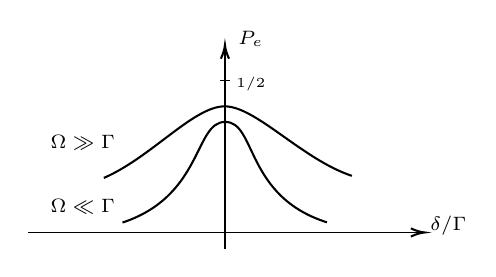
\begin{tikzpicture}[x=0.75pt,y=0.75pt,yscale=-1,xscale=1]
%uncomment if require: \path (0,122); %set diagram left start at 0, and has height of 122

%Curve Lines [id:da8052966326082212] 
\draw [line width=0.75]    (46.93,79.33) .. controls (69.93,69.33) and (90.17,44.83) .. (105.17,44.83) .. controls (120.17,44.83) and (142.43,70.33) .. (166.43,78.33) ;
%Straight Lines [id:da4526791024224187] 
\draw    (105.28,113.33) -- (105.28,17.33) ;
\draw [shift={(105.28,15.33)}, rotate = 90] [color={rgb, 255:red, 0; green, 0; blue, 0 }  ][line width=0.75]    (6.56,-1.97) .. controls (4.17,-0.84) and (1.99,-0.18) .. (0,0) .. controls (1.99,0.18) and (4.17,0.84) .. (6.56,1.97)   ;
%Straight Lines [id:da06360510795593066] 
\draw    (10.5,105.6) -- (199.43,105.6) ;
\draw [shift={(201.43,105.6)}, rotate = 180] [color={rgb, 255:red, 0; green, 0; blue, 0 }  ][line width=0.75]    (6.56,-1.97) .. controls (4.17,-0.84) and (1.99,-0.18) .. (0,0) .. controls (1.99,0.18) and (4.17,0.84) .. (6.56,1.97)   ;
%Straight Lines [id:da559598823855056] 
\draw    (103,32.5) -- (107.93,32.5) ;
%Curve Lines [id:da04885805308328728] 
\draw [line width=0.75]    (55.93,100.83) .. controls (94.93,87.83) and (90.43,52.33) .. (105.43,52.33) .. controls (120.43,52.33) and (114.93,88.22) .. (154.43,100.72) ;

% Text Node
\draw (203,96.4) node [anchor=north west][inner sep=0.75pt]  [font=\scriptsize]  {$\delta /\Gamma $};
% Text Node
\draw (109.5,29.4) node [anchor=north west][inner sep=0.75pt]  [font=\tiny]  {$1/2$};
% Text Node
\draw (20,57.4) node [anchor=north west][inner sep=0.75pt]  [font=\scriptsize]  {$\Omega \gg \Gamma $};
% Text Node
\draw (20,88.4) node [anchor=north west][inner sep=0.75pt]  [font=\scriptsize]  {$\Omega \ll \Gamma $};
% Text Node
\draw (110.5,7.2) node [anchor=north west][inner sep=0.75pt]  [font=\scriptsize]  {$P_{e}$};

\end{tikzpicture}
 }
\end{center}


\noindent From this expression, we recognize that two regimes are possible: 
\begin{itemize}
    \item weak drive: 
    \begin{align*}
        \Omega \ll \Gamma \qquad \implies \qquad P_e \simeq \frac{\Omega^2}{4 \delta^2 + \Gamma^2}, 
    \end{align*} 
    which is Lorentzian with width $\sim \Gamma$; 
    \item strong drive: 
    \begin{align*}
        \Omega \gg \Gamma \qquad \implies \qquad P_e \simeq \frac{\Omega^2}{4 \delta^2 + 2\Omega^2}, 
    \end{align*} 
    which is Lorentzian with width $\sim \Omega$; 
\end{itemize}

\section{Three-level atoms and Raman coupling}

Consider a three-level atom, with two quasi-ground states (meaning that they are very stable) $\ket{g_i}, i = 0,1\;$, and a short-lived excited state $\ket{e}$; assume that transitions between the quasi-ground states are forbidden. A schematic view is reported in figure \ref{fig:lambda}. 
\begin{figure}[h]
\centering
    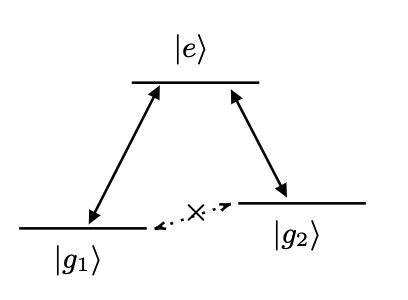
\includegraphics[width=0.3\linewidth]{images/lambda_system.png}
    \caption{$\Lambda$ system with suppressed transition between the ground states. }
    \label{fig:lambda}
\end{figure}

The Hamiltonian for the atom and for the atom-light interaction are 
\begin{align*}
H_{A} &= -\hbar \omega_{g_1} \ket{g_1}\bra{g_1} -\hbar \omega_{g_2} \ket{g_2}\bra{g_2} + 0\\
H_{AL} &= - \hat{\vec{d}} \cdot \hat{\vec{E}},
\end{align*}
where the dipole transition term evaluates as
\begin{equation*}
\begin{aligned}
{\vec{d}} = -e{\vec{r}}  ~\big\rvert_{g_1,g_2,e} & =  -e\ket{g_1}\bra{g_1}\vec{r}\ket{e}\bra{e} \;\;- e\ket{g_2}\bra{g_2}\vec{r}\ket{e}\bra{e} \;\; + \text{h.c.} \\
&\equiv d_{eg_1}^*\ket{g_1}\bra{e} \;\;+\;\; d_{eg_2}^*\ket{g_2}\bra{e} \;\; + \text{h.c}.
\end{aligned}
\end{equation*}
In this derivation, we will write the electric field is written in a slightly different way with respect to the previous chapters: 
\begin{equation*}
\vec{E} =
\sum_{\vec{k},\lambda} \sqrt{\frac{\hbar\omega_k}{2\varepsilon_0}}\vec\epsilon_{\lambda} \, 2 \mathfrak{Im} \left[u_{\vec{k},\lambda}(\vec{r}_\text{atom})\hat{a}_{\vec{k},\lambda}\right], 
\end{equation*}
since for a generic operator $A$ one can write $\mathfrak{Im} A = (A-A^\dagger)/2i$. Notice that $\vec{r}_\text{atom}$ is evaluated in center-of-mass coordinate and not in the coordinates of the electron. 

Consider two independent lasers to control the system
\begin{equation*}
\ket{\psi_\text{lasers}} = \ket{0} \otimes \dots \otimes \ket{0} \otimes \underbrace{\ket{\alpha_1}}_{\substack{\textrm{first laser}\\k_1,\lambda_1}} \otimes \ket{0} \otimes \dots \otimes \ket{0} \otimes \underbrace{\ket{\alpha_2}}_{\substack{\textrm{second laser}\\k_2,\lambda_2}} \otimes \ket{0} \otimes \dots,
\end{equation*}
and assume that: 
\begin{itemize}
    \item $\vec{E}$ is perceived by the system as an averaged value
    \begin{align*}
    \bra{\psi_\text{lasers}}\vec{E}\ket{\psi_\text{lasers}} & = \sqrt{\frac{\hbar\omega_1}{2 \varepsilon_0}}
\vec\epsilon_{\lambda_1} 2 \mathfrak{Im} \left(u_{\vec{k}_1,\lambda_1}\right) \bra{\alpha_1}\hat{a}_{\vec{k}_1,\lambda_1} \ket{\alpha_1} + \left(\substack{\text{same for}\\\vec{k}_2, \lambda_2 }\right)\\ 
& = \sqrt{\frac{2\hbar\omega_1}{\varepsilon_0}}
\vec\epsilon_{\lambda_1} |u_{\vec{k}_1,\lambda_1}||\alpha_1| \cos\left[(c k_1)t + \phi_1\right] + \left(\substack{\text{same for}\\\vec{k}_2, \lambda_2 }\right),
    \end{align*}
    \item the lasers are powerful and hence the state $\ket{\psi}_\text{laser}$ is not much affected by the absorption of one photon.
\end{itemize}
The average value of the electric field can be rewritten as  
    \begin{align}
        \langle \vec{E}\rangle =
\vec{\mathcal{E}}_1 \cos\left(\omega_1t + \phi_1\right) +
\vec{\mathcal{E}}_2 \cos\left(\omega_2t + \phi_2\right). 
    \end{align}
From the previous considerations
\begin{align*}
    H_{AL} & = - \hat{\vec{d}} \cdot \langle \vec{E}\rangle = \\
    &= -\left(
    \vec{d}_{eg_1}\ket{e}\bra{g_1} \;+\; 
    \vec{d}_{eg_2}\ket{e}\bra{g_2} \;+\; 
    \vec{d}_{eg_1}^*\ket{g_1}\bra{e} \;+\; 
    \vec{d}_{eg_2}^*\ket{g_2}\bra{e}
\right)
\cdot\\
&\qquad \cdot\left(
    \vec{\mathcal{E}}_1 \cos\left(\omega_1t + \phi_1\right)
    \;+\;
    \vec{\mathcal{E}}_2 \cos\left(\omega_2t + \phi_2\right)
\right). 
\end{align*}
A formal simplification can be done by introducing the the coefficients
\begin{equation*}
      \Omega_1 = \frac{\vec{d}_{eg_1} \cdot \vec{\mathcal{E}}_1}{\hbar}
      \qquad\qquad
      \Omega_2 = \frac{\vec{d}_{eg_2} \cdot \vec{\mathcal{E}}_1}{\hbar}
\end{equation*}
\begin{equation*}
    \cancel{\Omega}_1 = \frac{\vec{d}_{eg_1} \cdot \vec{\mathcal{E}}_2}{\hbar}
    \qquad\qquad
    \cancel{\Omega}_2 = \frac{\vec{d}_{eg_2} \cdot \vec{\mathcal{E}}_2}{\hbar}
\end{equation*}
in order to write
\begin{align*}
    H_{AL} &= -\hbar \bigg[ \ket{e}\bra{g_1} \left( \Omega_1 \cos{(\omega_1 t + \phi_1)} + \cancel{\Omega}_1 \cos{(\omega_2 t + \phi_2)}\right) + \\
    &~~~+ \ket{e}\bra{g_2} \left( \Omega_2 \cos{(\omega_2 t + \phi_2)} + \cancel{\Omega}_2 \cos{(\omega_1 t + \phi_1)}\right) + \text{h.c.} \bigg] 
\end{align*}

Eventually, the full Hamiltonian in the laboratory frame, sorting the basis in the order $\{\ket{g_1}, \ket{e}, \ket{g_2}\}$, is
\begin{equation*}
H^{lab} = -\hbar \left(
    \begin{array}{c;{5pt/5pt}c;{5pt/5pt}c}
    \omega_{eg_1} & \text{c.c.} & 0\\ \hdashline[5pt/5pt]
    \Omega_1\cos\left(\omega_1t + \phi_1\right) + 
     & \multirow{2}{*}{0} & \multirow{2}{*}{\text{c.c.}}\\
    + \cancel{\Omega}_1\cos\left(\omega_2t + \phi_2\right) &&\\ \hdashline[5pt/5pt]
    \multirow{2}{*}{0}& \Omega_2^*\cos\left(\omega_2t + \phi_2\right) + & \multirow{2}{*}{$\omega_{eg_2}$}\\
    &+\cancel{\Omega}_2^*\cos\left(\omega_1t + \phi_1\right)&\hspace*{3cm}
    \end{array}
\right)
\end{equation*}
Now a change of reference frame is performed, for convenience,
$$H^{lab} \quad \longrightarrow \quad H^{rot} = U H^{lab}U^\dagger + i \hbar \dot{U} U^\dagger,$$
applying the time-dependent rotation
\begin{equation*}
U(t) = \begin{pmatrix}
e^{-i(\omega_1t + \phi_1)} & 0 & 0\\
0 & 1 & 0\\
0 & 0 & e^{-i(\omega_2t + \phi_2)}
\end{pmatrix}
\;\; .
\end{equation*}
Hence, the two terms composing the rotated hamiltonian are
\begin{align*}
UH^{lab}U^\dag & = - \hbar U
\begin{pmatrix}
\omega_{eg_1}e^{i(\omega_1...)} & (\Omega_1 ... + \cancel{\Omega}_1...) & 0\\
(\Omega_1 ... + \cancel{\Omega}_1...)e^{i(\omega_1...)} & 0 & (\Omega_2 ... + \cancel{\Omega}_2...)e^{i(\omega_2...)}\\
0 & (\Omega_2 ... + \cancel{\Omega}_2...) & \omega_{eg_2}e^{i(\omega_2...)}\\
\end{pmatrix}
\end{align*}
and 
\begin{equation*}
i\hbar\dot{U}U^\dag = \hbar
\begin{pmatrix}
\omega_1 & 0 & 0\\
0 & 0 & 0\\
0 & 0 & \omega_2
\end{pmatrix}.
\end{equation*}
The final result is
\begin{equation*}
H_{rot} = -\hbar \left(
    \begin{array}{ccc}
    \omega_{eg_1} -\omega_1 & \text{c.c.} & 0\\ %\hdashline[6pt/6pt]
    (\Omega_1 ... + \cancel{\Omega}_1...)e^{i(\omega_1t+\phi_1)}
     & 0 & \text{c.c.}\\ %\hdashline[6pt/6pt]
    0 & (\Omega_2 ... + \cancel{\Omega}_2...)e^{-i(\omega_2t+\phi_2)} & \omega_{eg_2}-\omega_2\\
    \end{array}
\right)
\end{equation*}
The following step consists of defining $\delta_1 \equiv \omega_{eg_1} -\omega_1$ and $\delta_2 \equiv \omega_{eg_2} -\omega_2$ and in breaking the full Hamiltonian in two pieces such that
$$H(t) = H_0 + V(t)$$
It is trivial that
\begin{align*}
H_0 & = - \hbar 
\begin{pmatrix}
\delta_1 & \Omega_1^*/2 & 0\\
\Omega_1/2 & 0 & \Omega_2/2\\
0 & \Omega_2^*/2 & \delta_2\\
\end{pmatrix}
\end{align*}
and 
\begin{align}
V(t)  = -\hbar \left(
    \begin{array}{c;{6pt/6pt}c;{6pt/6pt}c}
    0 & \text{c.c.} & 0 \\ \hdashline[6pt/6pt]
    \dfrac{\Omega_1}{2} e^{2i(\omega_1t+\phi_1)} + 
     & \multirow{4}{*}{0} & \multirow{4}{*}{\text{c.c.}}\\
     + \dfrac{\cancel{\Omega}_1}{2} e^{i(\omega_1+\omega_2)t} e^{i(\phi_1+\phi_2)} + & & \\
     + \dfrac{\cancel{\Omega}_1}{2} e^{i(\omega_1-\omega_2)t} e^{i(\phi_1-\phi_2)} & & \\\hdashline[6pt/6pt]
    \multirow{2}{*}{0} & \text{something}& \multirow{2}{*}{0} \\
    & \text{similar} &
    \end{array}
\right)
\end{align}

As we already know, this formulation allows to describe the problem in terms of an effective Hamiltonian
\begin{equation}
H_{\text{eff}} = H_0 + 
\frac{1}{\hbar \tilde\omega}\left[V,V^\dag\right] + \mathcal{O}(\omega^{-2})
\label{eq:ch6:lambdaform}
\end{equation}
where $\tilde{\omega}$ is the oscillation frequency of $V(t)$. The term ${1}/(\hbar {\tilde\omega}) \left[V,V^\dag\right]$ could be neglected if the timescales of $H_0$ are much larger than ${1}/{\tilde\omega}$ or equivalently, if the energy scales of $H_0$ ($\Omega_1$, $\Omega_2$, $\delta_1$, $\delta_2$) and $V$ ($\cancel{\Omega}_1$, $\cancel{\Omega}_2$) are much smaller than $\hbar\tilde\omega$. \\
Basically, this implies that
$$\Omega_1,\; \Omega_2,\; \cancel{\Omega_1},\; \cancel{\Omega_2}, |\delta_1|,\; |\delta_2| ~
\ll ~\omega_1,\; \omega_2,\; \omega_1+\omega_2,\; |\omega_1-\omega_2|.$$
The most strict bound is on $|\omega_1-\omega_2|$, which physically means that the frequencies of the two lasers can not be too close. 
% By a physical point of view, this condition is met if $g_1$ and $g_2$ are not too close!

Adding a constant $\hbar\delta_1$, and neglecting the second term of equation (\ref{eq:ch6:lambdaform}), the effective Hamiltonian of the system is
\begin{equation*}
H_{\text{eff}} = H_0 = \hbar \begin{pmatrix}
    0 & \bigg\rvert\dfrac{\Omega_1}{2}\bigg\rvert & 0\\
    \bigg\rvert\dfrac{\Omega_1}{2}\bigg\rvert & \delta_1 & \bigg\rvert\dfrac{\Omega_2}{2}\bigg\rvert\\
    0 & \bigg\rvert\dfrac{\Omega_2}{2}\bigg\rvert & \Delta
\end{pmatrix}
\end{equation*}
where $\Delta \equiv \delta_1 - \delta_2$ and $\ket{e}$. Adding a phase to $\ket{e}$, it is possible to obtain real values for $\Omega_1$ and $\Omega_2$. 

Finally, in order for this problem to be equivalent to the previously solved three-level problem (section \ref{sec:timedep}), we must make additional hypothesis:
$$ \Delta, \Omega_j \ll \delta_j \qquad \qquad j = 1, 2.$$
\begin{tcolorbox} [breakable, enhanced]
The hypothesis constraints are usually met in the experiments with these timescales:
\begin{equation*}
\underbrace{\Delta, \Omega_j}_{\sim MHz} \;
\ll 
\underbrace{|\delta_1|,\;|\delta_2|}_{\sim GHz}
\ll 
\underbrace{\omega_1,\;\omega_2,\;|\omega_1-\omega_2|}_{ \sim THz}
\end{equation*}
\end{tcolorbox}

\noindent Now the problem is formally equivalent to the $\Lambda$-system. The time-independent second-order perturbation theory can be applied considering
\begin{equation*}
H_\text{unpert} = \hbar \begin{pmatrix}
    0 & 0 & 0\\
    0 &\delta_1 \simeq \delta_2 & 0\\
    0 & 0 & 0
\end{pmatrix} 
\end{equation*}
and 
\begin{equation*}
H_\text{pert}^{(A)} = 
\frac{\hbar}{2}\begin{pmatrix}
    0&\Omega_1&0\\
    \Omega_1&0&\Omega_2\\
    0&\Omega_2&0
\end{pmatrix}
\qquad\qquad
H_\text{pert}^{(B)} = 
\hbar\begin{pmatrix}
    0 & 0 & 0\\
    0 & 0 & 0\\
    0 & 0 & \Delta
\end{pmatrix}.
\end{equation*}
The final Hamiltonian projected on the ground state space is 
\begin{equation*}
\begin{aligned}
H_\text{final}^{\ket{g_1}\ket{g_2}} &= -\frac{\hbar}{4\delta}
\begin{pmatrix}
\Omega_1^2 & \Omega_1\Omega_2\\
\Omega_1\Omega_2 & \Omega_2^2
\end{pmatrix} + \hbar
\begin{pmatrix}
    0&0\\
    0&\Delta
\end{pmatrix} = \\
&=
-\hbar \frac{\Omega_1\Omega_2}{4\delta}\sigma_x
+\hbar\left(
\frac{\Omega_2^2 - \Omega_1^2}{8\delta}-\Delta
\right) \sigma_z + \text{const}. 
\end{aligned}
\end{equation*}




From the practical point of view, the systems transits between the ground states by absorbing and emitting a photon at the same time (one by each laser, at different frequencies). \\

The following sections will explain how to move to an environment with many atoms. 
